\documentclass[a4paper]{article}

\usepackage[english]{babel}
\usepackage{amsmath}
\usepackage{amssymb}
\usepackage{dsfont}
\usepackage{graphicx}
\usepackage{listings}
\usepackage[hyphens]{url}
\usepackage{pgf, tikz}
\usetikzlibrary{arrows, automata}
\usepackage{titling}
\usepackage{varwidth}
\usepackage{hyperref}
\usepackage{color} %red, green, blue, yellow, cyan, magenta, black, white
\definecolor{mygreen}{RGB}{28,172,0} % color values Red, Green, Blue
\definecolor{mylilas}{RGB}{170,55,241}
\setlength\parindent{0pt}

\newcommand\independent{\protect\mathpalette{\protect\independenT}{\perp}}
\def\independenT#1#2{\mathrel{\rlap{$#1#2$}\mkern2mu{#1#2}}}

\usepackage{geometry}
 \geometry{
 a4paper,
 total={165mm,257mm},
 left=20mm,
 top=20mm,
 }

\title{Statistical Machine Learning 2018\\Assignment 1\\Deadline: 7th of October 2018}
\author{
  Christoph Schmidl\\ s4226887\\      \texttt{c.schmidl@student.ru.nl}
  \and
  Mark Beijer\\ s4354834\\     \texttt{mbeijer@science.ru.nl}
}
\date{\today}

\begin{document}
\maketitle


\section*{Exercise 1 - weight 5}

Consider once more the M-th order polynomial

\begin{equation}
	y(x;w) = w_0 + w_1x + ... + w_Mx^M = \sum_{j = 0}^M w_jx^j
\end{equation}

\subsection*{1.1}

Create the function $f(x) = sin(6(x-2))$ in MATLAB. Generate a data set $\mathcal{D}_{10}$ of 10 noisy observation of this function. Take the 10 inputs spaced uniformly in range $[0,1]$, and assume that the noise is gaussian with mean 0 and standard deviation 0.3. $\mathcal{D}_{10}$ will be the training set. In a similar way, generate an additional test set $\mathcal{T}$ of 100 noisy observations over the same interval. plot both the function and observation in $\mathcal{D}_{10}$ in a single graph (similar to Bishop, Fig.1.2).\\

\textbf{Answer:}\\

\subsection*{1.2}

Create a MATLAB function $w = PolCurFit(\mathcal{D}_N,M)$ that takes as input a data set $\mathcal{D}_N$, consisting of $N$ input/output-pairs $\{ x_n, t_n\}$, and a parameter $M$, representing the order of the polynomial in (1), and outputs a vector of weights $w = [w_0, ...,w_M]$ that minimizes the sum-of-squares error function

\begin{equation}
	E(w) = \frac{1}{2} \sum_{n=1}^N \{ y(x_n;w) - t_n\}^2
\end{equation}

Hint: use the results from the Tutorial Exercises (Week1, Exercise 5), and the \textbackslash-operator (backslash) in MATLAB to solve a linear system of equations.\\

\textbf{Answer:}\\

\subsection*{1.3}

For the given dataset $\mathcal{D}_{10}$, run the $PolCurFit()$ function for $M = [0,...,9]$, and,

\begin{itemize}
	\item Plot for various orders $M$ (at least for $M = 0, M = 1, M = 3, M = 9$) the resulting ploynomial, together with the function $f$ and observation $\mathcal{D}_{10}$ (similar to Bishop, Fig 1.4)
	\item For each order $M \in [0,...,9]$, compute the root-mean-square error
	
	\begin{equation}
		E_{RMS} = \sqrt{2E(w^*)/N}
	\end{equation}
	
	of the corresponding polynomial, evaluated on both the training set $\mathcal{D}_{10}$ and the test set $\mathcal{T}$. Plot both as a function of $M$ in a single graph. (see Bishop, Fig.1.5).\\
\end{itemize}

\textbf{Answer:}\\



\subsection*{1.4}


Repeat this procedure for a data set $\mathcal{D}_{40}$ of 40 observations (with the same noise level) and compare with the previous result.\\

\textbf{Answer:}\\


\subsection*{1.5}

Modify the $PolCurFit()$ function to include an additional penalty parameter $\lambda$, for a procedure that solves the minimization problem for a modified error function with quadratic regularizer (weight decay), given as 

\begin{equation}
	\widetilde{E} = E + \frac{\lambda}{2} \sum_{j = 0}^M w_j^2
\end{equation}

Verify that the regularizer drives the weights of high order terms in the polynomial to zero, and see if you can reproduce the explain the effect observed in Bishop, Fig.1.8.\\

\textbf{Answer:}\\


\subsection*{1.6}

The polynomial curve fitting procedure can be extened to the case of multidimensional inputs. Assuming an input vector of dimension $D$, namely $x = (x_1,x_2,...,x_D)$, we can write the regression function $y$ as:

\begin{equation}
	y(x;w) = \sum_{j=0}^M \Bigg( \sum_{n_1+n_2+...n_D=j} w_{n_1 n_2...n_D}x_1^{n_1}x_2^{n_2} ... x_D^{n_D}\Bigg)
\end{equation}

In the last expression, $j$ refers to the order of the polynomial terms. The inner sum is over all the combinations of non-negative integers $n_1, n_2, ..., n_D$, such that the constraint $n_1+ n_2 + ... + n_D = j$ holds. The terms $n_1, n_2,..., n_D$ correspond to the exponent for each variable $x_1,x_2,...,x_D$ in their respective polynomial term.\\

Note that if $D = 1$, the above expression simplifies to the formula in Equation (1). The reason the second sum disappears is that there is only one combination of the non-negative integer $n_1$ for which the constraint $n_1 = j$ holds, which means that there is only a single term to sum over.\\

Fitting the polynomial curve to a multidimensional input vector works analogously to the one-dimensional case. However, the number of parameters (the size of w) becomes much larger, even when $D = 2$. Write down the general polynomial curve equation in (5) for $D = 2$. How many parameters are needed in the two-dimensional case? Compare this to the number of parameters in the one-dimensional case.\\


\textbf{Answer:}\\

\section*{Exercise 2 - weight 2.5}

In this exercise, we consider the gradient descent algorithm for function minimization. When the function to be minimized $E(x)$, the gradient descent iteration is

\begin{align*}
	x_{n+1} = x_n - \eta \nabla E(x_n)
\end{align*}

where $\eta > 0$ is the so-called learning rate. In the following, we will apply gradient descent to the function

\begin{align*}
	h(x,y) = 100(y - x^2)^2 + (1 - x)^2
\end{align*}

\subsection*{2.1}

Make a plot of the function $h$ over the interval $[-2 \leq x \leq 2] \times [-1 \leq y \leq 3]$. Tip: use MATLAB function \textbf{surf}. Can you guess from the plot if numerical minimization with gradient descent will be fast or slow for this function?\\

\textbf{Answer:}\\

\subsection*{2.2}

Knowing that a critical point of a function is a point where the gradient vanishes, show that $(1,1)$ is the unique critical point og $h$. Prove that this point is a minimum for $h$.\\

\textbf{Answer:}\\


\subsection*{2.3}

Write down the gradient descent iteration rule for this function.

\textbf{Answer:}\\


\subsection*{2.4}

Implement gradient descent in MATLAB. Try some different values of $\eta$. Does the algorithm converge? How fast? Make plots of the trajectories on top of a contour plot of $h$. (Hint: have look at the MATLAB example code $contour\_example.m$ on Brightspace for inspiration to plot contours of functions and trajectories). Report your findings. Explan why numerical minimization with gradient descent is slow for this function.\\

\textbf{Answer:}\\


\section*{Exercise 3 - weight 2.5}


Suppose we have two healthy but curiously mixed boxes of fruit, with one box containing 8 apples and 4 grapefruits and the other containing 15 apples and 3 grapefruits. One of the boxes is selected at random and a piece of fruit is picked (but not eaten) from the chosen box, with equal probability for each item in the box. The piece of fruit is returned and then once again from the \textit{same} box a second piece is chosen at random. This is known as sampling with replacement. Model the box by random variable $\boldsymbol{B}$, the first piece of fruit by variable $\boldsymbol{F_1}$, and the second piece by $\boldsymbol{F_2}$.


\subsection*{3.1}

\textbf{Question:} What is the probability that the first piece of fruit is an apple given that the second piece of fruit was a grapefruit? How can the result of the second pick affect the probability of the first pick?\\

\textbf{Answer:}\\

Let's define the two random variables more specifically to later on save some writing. 

\begin{align*}
	B &= \{ 1,2\}\\
	F &= \{ A,G \}\\
	F_1 &= \texttt{First piece of fruit}\\
	F_2 &= \texttt{Second piece of fruit}
\end{align*}

The random variable $B$ (for Box) can take the values $1$ or $2$ for Box 1 or Box 2 respectively.\\
The random variable $F$ (for fruit) can take the values $A$ or $G$ for Apple or Grapefruit respectively.\\ 

Box 1 contains:

\begin{itemize}
	\item 8 apples
	\item 4 grapefruits
	\item 12 fruits in total
\end{itemize}

Box 2 contains :

\begin{itemize}
	\item 15 apples
	\item 3 grapefruits
	\item 18 fruits in total
\end{itemize}

To answer the question we have to find the following probability:

\begin{align*}
	p(F_1 = A | F_2 = G)\\	
\end{align*}



The tricky part is due to the fact that the piece of fruit is returned and then once again from the \textit{same} box a second piece is chosen at random. Otherwise we could just apply Bayes' theorem and would be done. Therefore we have to calculate the probability to pick a grapefruit or apple from each box separately.

\begin{align*}
	p(F = A | B = 1) &= \frac{2}{3}\\
	p(F = A | B = 2) &= \frac{5}{6}\\
	p(F = G | B = 1) &= 1 - p(F = A | B = 1) = 1 - \frac{2}{3} = \frac{1}{3}\\
	p(F = G | B = 2) &= 1 - p(F = G | B = 2) = 1 - \frac{5}{6} = \frac{1}{6}\\
	p(F = G) &= \frac{1}{3} \times \frac{1}{2} + \frac{1}{6} \times \frac{1}{2} = \frac{1}{4}
\end{align*}

\begin{align*}
	p(B = 1 | F = G) = \frac{p(F = G | B = 1)p(B = 1)}{p(F = G)} = \frac{\frac{1}{3} \times \frac{1}{2}}{\frac{1}{4}} = \frac{2}{3}\\
	p(B = 2 | F = G) = \frac{p(F = G | B = 2)p(B = 2)}{p(F = G)} = \frac{\frac{1}{6} \times \frac{1}{2}}{\frac{1}{4}} = \frac{1}{3}
\end{align*}

Now we can calculate the probability of each box:

\begin{align*}
	p(F_1 = A | F_2 = G) &= p(B = 1| F = G)p(F = A | B = 1) + p(B = 2 | F = G)p(F = A | B = 2)\\
	&= \frac{2}{3} \times \frac{2}{3} +  \frac{1}{3} \times \frac{5}{6}	\\
	&= \frac{4}{9} \times \frac{5}{18}\\
	&= \frac{13}{18} \approx 0.722
\end{align*}

The probability that the first fruit is an apple given that the second fruit is a Grapefruit picked from the same box as the apple is $\frac{13}{18}$.\\
The probability that the first fruit is an apple given that the second fruit is a grapefruit and both are picked from Box 1 is $\frac{8}{18}$, whereas the probability that the first fruit is an apple given that the second fruit is a grapefruit and both are picked from Box 2 is $\frac{5}{18}$. Therefore the second pick affects the probability of the first pick in such a way that is gives us a clue about the box it was picked from.

\subsection*{3.2}


\textbf{Question:} Imagine now that after we remove a piece of fruit, it is not returned to the box. This is known as sampling without replacement. In this situation, recompute the probability that the first piece of fruit is an apple given that the second piece of fruit was a grapefruit. Explain the difference.\\

\textbf{Answer:}\\

We want to find the following probability based on sampling without replacement:

\begin{align*}
	P(F_1 = A | F_2 = G)
\end{align*}

We have to extend the original formula from the previous exercise:

\begin{align*}
	p(F_1 = A | F_2 = G) &= p(B = 1| F = G)p(F = A | B = 1) + p(B = 2 | F = G)p(F = A | B = 2)\\
\end{align*}

And add the case for sampling without replacement. Therefore, the order of the pick is now important and the amount of fruits in a box changes accordingly:

\begin{align*}
	p(F_1 = A | B = 1) &= \frac{2}{3}\\
	p(F_1 = A | B = 2) &= \frac{5}{6}\\
	p(F_2 = G | B = 1) &= \frac{4}{11}  \quad \texttt{Removed one apple from box 1}\\
	p(F_2 = G | B = 2) &= \frac{3}{17} \quad \texttt{Removed one apple from box 2}\\
		p(F_2 = G) &= \frac{4}{11} \times \frac{1}{2} + \frac{3}{17} \times \frac{1}{2} = \frac{101}{374}
\end{align*}

\begin{align*}
	p(B = 1 | F_2 = G) = \frac{p(F_2 = G | B = 1)p(B = 1)}{p(F_2 = G)} = \frac{\frac{4}{11} \times \frac{1}{2}}{\frac{101}{374}} = \frac{68}{101}\\
	p(B = 2 | F_2 = G) = \frac{p(F_2 = G | B = 2)p(B = 2)}{p(F_2 = G)} = \frac{\frac{3}{17} \times \frac{1}{2}}{\frac{101}{374}} = \frac{33}{101}
\end{align*}

\begin{align*}
	p(F_1 = A | F_2 = G) &=   p(B = 1| F_2 = G)p(F_1 = A | B = 1) + p(B = 2 | F_2 = G)p(F_1 = A | B = 2)\\
	&= \frac{68}{101} \times \frac{2}{3} + \frac{33}{101} \times \frac{5}{6}\\
	&= \frac{437}{606} \approx 0.72112
\end{align*}

The difference between the probabilities of exercise 3.1 and exercise 3.2 are so minimal that they are nearly the same or not really significant. In the previous exercise the probability of $P(F_1 = A | F_2 = G)$ was $\frac{13}{18}$ which is $\approx 0.72$. In this exercise the probability of $P(F_1 = A | F_2 = G)$ was $\frac{437}{606}$ which is $\approx 0.72112$. The main difference is based on the fact that the total amount of fruits in a box changes after the first pick from either 12 to 11 for Box 1 or from 18 to 17 for Box 2. Because the removed fruit in the first pick is already fixed to being an apple, the probabilities of picking a grapefruit from the reduced amount of total fruits is minimal.


\subsection*{3.3}

\textbf{Question:} Starting from the initial situation (i.e.,sampling with replacement), we add a dozen oranges to the first box and repeat the experiment. Show that now the outcome of the first pick has no impact on the probability that the second pick is a grapefruit. Are the two picks now dependent or independent? Explain your answer.\\

\textbf{Answer:}\\

If we add a dozen (12) oranges to Box 1 then the total distribution among the boxes looks as follows:

Box 1 contains:

\begin{itemize}
	\item 8 apples
	\item 4 grapefruits
	\item 12 oranges
	\item 24 fruits in total
\end{itemize}

Box 2 contains :

\begin{itemize}
	\item 15 apples
	\item 3 grapefruits
	\item 18 fruits in total
\end{itemize}

In order to show that the outcome of the first pick has no impact on the probability that the second pick is a grapefruit, We have to show that

\begin{align*}
	p(F_2 = G | F_1 = A) = p(F_2 = G | F_1 = G) = p(F_2 = G | F_1 = O)\\
\end{align*}

\begin{align*}
	p(F = A | B = 1) &= \frac{1}{3}\\
	p(F = A | B = 2) &= \frac{5}{6}\\
	p(F = G | B = 1) &= \frac{1}{6}\\
	p(F = G | B = 2) &= \frac{1}{6}\\
	p(F = O | B = 1) &=  \frac{1}{2}\\
	p(F = O | B = 2) &=  0\\
	p(F = G) &= \frac{1}{6} \times \frac{1}{2} + \frac{1}{6} \times \frac{1}{2} = \frac{1}{6}\\
	p(F = A) &= \frac{1}{3} \times  \frac{1}{2} + \frac{5}{6} \times \frac{1}{2} = \frac{7}{12}\\
	p(F = O) &= \frac{1}{2} \times \frac{1}{2} + 0 \times \frac{1}{2} =  \frac{1}{4}
\end{align*}

\begin{align*}
	p(B = 1 | F = G) = \frac{p(F = G | B = 1)p(B = 1)}{p(F = G)} = \frac{\frac{1}{6} \times \frac{1}{2}}{\frac{1}{6}} = \frac{1}{2}\\
	p(B = 2 | F = G) = \frac{p(F = G | B = 2)p(B = 2)}{p(F = G)} = \frac{\frac{1}{6} \times \frac{1}{2}}{\frac{1}{6}} = \frac{1}{2}
\end{align*}

Calculating $p(F_2 = G | F_1 = A)$:

\begin{align*}
	p(F_1 = A | F_2 = G) &= p(B = 1| F = G)p(F = A | B = 1) + p(B = 2 | F = G)p(F = A | B = 2)\\
	&= \frac{1}{2} \times \frac{1}{3} +  \frac{1}{2} \times \frac{5}{6}\\
	&= \frac{7}{12}
\end{align*}


\begin{align*}
	p(F_2 = G | F_1 = A) = p(F_2 = G | F_1 = G) = p(F_2 = G | F_1 = O)\\
\end{align*}


\begin{align*}
	p(F_2 = G | F_1 = A) &= \frac{p(F_1 = A | F_2 = G)p(F_2 = G)}{p(F_1 = A)}\\
	&= \frac{\frac{7}{12} \times \frac{1}{6}}{\frac{7}{12}}\\
	&= \frac{1}{6}
\end{align*}


Calculating $p(F_2 = G | F_1 = G)$:

\begin{align*}
	p(F_1 = G | F_2 = G) &=  p(B = 1| F = G)p(F = G | B = 1) + p(B = 2 | F = G)p(F = G | B = 2)\\
	&= \frac{1}{2} \times \frac{1}{6} + \frac{1}{2} \times \frac{1}{6}\\
	&= \frac{1}{6}
\end{align*}

\begin{align*}
	p(F_2 = G | F_1 = G) &= \frac{p(F_1 = G | F_2 = G)p(F_2 = G)}{p(F_1 = G)}\\
	&= \frac{\frac{1}{6} \times \frac{1}{6}}{\frac{1}{6}}\\
	&= \frac{1}{6}
\end{align*}


Calculating $p(F_2 = G | F_1 = O)$:

\begin{align*}
	p(F_1 = O | F_2 = G) &= p(B = 1| F = G)p(F = O | B = 1) + p(B = 2 | F = G)p(F = O | B = 2)\\
	&= \frac{1}{2} \times \frac{1}{2} +  \frac{1}{2} \times 0\\
	&= \frac{1}{4}
\end{align*}

\begin{align*}
	p(F_2 = G | F_1 = O) &= \frac{p(F_1 = O | F_2 = G)p(F_2 = G)}{p(F_1 = O)}\\
	&= \frac{\frac{1}{4} \times \frac{1}{6}}{\frac{1}{4}}\\
	&= \frac{1}{6}
\end{align*}

Therefore the statement holds that:

\begin{align*}
p(F_2 = G | F_1 = A) &= p(F_2 = G | F_1 = G) = p(F_2 = G | F_1 = O)\\
\frac{1}{6} &= \frac{1}{6} = \frac{1}{6}
\end{align*}

The two picks are independent because the pick of the first fruit does not affect the pick of the second fruit and the probability is equal amongst the picks.

\section*{Exercise 4 - Bonus (weight 1)}

Given a joint probability function over the random vector $X = (X_1, X_2, X_3, X_4)$ that factorizes as

\begin{align*}
	p(x_1,x_2,x_3,x_4) = p(x_1,x_4|x_2)p(x_2,x_3|x_1)
\end{align*}

show (using the sum and product rules for marginals and conditionals) that the following independence statements hold:

\subsection*{4.1}

\begin{align*}
	X_1 \independent X_2
\end{align*}


\textbf{Answer:}\\

In order to show that $X_1 \independent X_2$, we have to prove that $p(x_1, x_2) = p(x_1)p(x_2)$. Figure \ref{fig:directed_graph} gives a visual representation of the factorization as a directed graph. We can already see that the statement $X_1 \independent X_2$ does not hold.


\begin{figure}[h]
\centering
    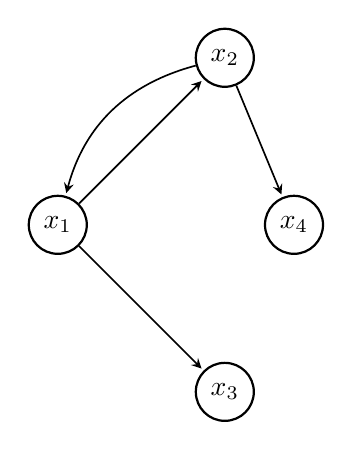
\begin{tikzpicture}[
            > = stealth, % arrow head style
            shorten > = 1pt, % don't touch arrow head to node
            auto,
            node distance = 3cm, % distance between nodes
            semithick % line style
        ]

        \tikzstyle{every state}=[
            draw = black,
            thick,
            fill = white,
            minimum size = 4mm
        ]

        \node[state] (x_1) {$x_1$};
        \node[state] (x_2) [above right of=x_1] {$x_2$};
        \node[state] (x_3) [below right of=x_1] {$x_3$};
        \node[state] (x_4) [right of=x_1] {$x_4$};
        

        \path[->] (x_1) edge node {} (x_2);
        \path[->] (x_2) edge[bend right] node {} (x_1);
        \path[->] (x_1) edge node {} (x_3);
        \path[->] (x_2) edge node {} (x_4);
      

    \end{tikzpicture}
\caption{Factorization as directed graph} \label{fig:directed_graph}
\end{figure}

We can rewrite the factorization as follows:

\begin{align*}
	p(x_1,x_2,x_3,x_4) &= p(x_1,x_4|x_2)p(x_2,x_3|x_1)\\
	&= p(x_1|x_2)p(x_4|x_2)p(x_2|x_1)p(x_3|x_1)
\end{align*}

We can now marginalize $x_1$ and $x_2$ and apply the sum and product rule at the end to get the joint probabilities:

\begin{align*}
	p(x_1) = p(x_1|x_2)p(x_2) = p(x_2, x_1)\\
	p(x_2) = p(x_2|x_1)p(x_1) = p(x_1, x_2)
\end{align*}

Therefore:

\begin{align*}
	p(x_1)p(x_2) = p(x_1,x_2)p(x_2,x_1)\\
	p(x_1, x_2) \neq p(x_1)p(x_2)
\end{align*}

Based on this contradiction the statement $X_1 \independent X_2$ does \textbf{not} hold.

\subsection*{4.2}

\begin{align*}
	X_3 \independent X_4 | X_1,X_2
\end{align*}

\textbf{Answer:}\\

In order to show that $X_3 \independent X_4 | X_1,X_2$, we have to prove that $p(x_3, x_4 | x_1, x_2) = p(x_3 | x_1, x_2)p(x_4 | x_1, x_2)$. 

We already know from the previous exercise that 

\begin{align*}
	p(x_1)p(x_2) = p(x_1,x_2)p(x_2,x_1)
\end{align*}

and based on the symmetry property we know that:

\begin{align*}
	p(x_1,x_2) = p(x_2,x_1)
\end{align*}

We can therefore replace the joint probabilities with marginal probabilities which makes it easier to prove the conditional independence:

\begin{align*}
	p(x_1,x_2) = p(x_1)\\
	p(x_1,x_2) = p(x_2)
\end{align*}

We can rewrite the statements as follows when we replace $p(x_1,x_2)$ for $p(x_1)$:

\begin{align*}
p(x_3, x_4 | x_1, x_2) = p(x_3 | x_1, x_2)p(x_4 | x_1, x_2)\\
p(x_3,x_4|x_1) = p(x_3|x_1)p(x_4|x_1)\\
p(x_3|x_1)p(x_4|x_1) = p(x_3|x_1)p(x_4|x_1)
\end{align*}

Therefore the statement $X_3 \independent X_4 | X_1,X_2$ holds.

\end{document}
